\documentclass[main.tex]{subfiles}

\title{The model for observing infections}
\author{Joshua Blake}
\date{\today}

\begin{document}
\maketitle

\section{Introduction}\label{introduction}

This paper discusses a model for observing duration of PCR positivity in
the Coronavirus (COVID-19) Infection Survey (CIS). The CIS continually
enrols individuals and tests them on an ongoing basis, following a
specified testing protocol. The protocol specifies that the initial five
tests are spaced every 7 days, then the spacing is every 28 days.
However, real-world considerations often lead to variations in test
times and missed tests. Our analysis focuses solely on the binary result
(positive or negative) of these tests, assuming no misclassification
bias

Two major challenges arise when dealing with this data: double interval
censoring and left truncation. Double interval censoring arises because
we can only bound the start and end of an infection by observing an
individual's test results transitioning from negative to positive and
vice versa. Left truncation occurs because an individual is infected at
time $t$ is only observed if their infection duration is at least
$t^N - t$ days long, where $t^N$ is the time of their next test.

To address these challenges, we employ two distinct approaches: the
``individual'' model and the ``total'' model.

The individual model considers only individuals with observed (i.e., not
truncated) episodes. This approach is similar to methods used in
previous studies, such as \textcite{heiseyModelling},
\textcite{dempsterMaximum}, and
\textcite{turnbullEmpirical}. The conceptual
approach here is to form a cohort of individuals for which we observe at
least one positive test, and then consider a study which had only
enrolled these individuals. The modelling approach then corrects for
this selection bias.

In contrast, the total model also takes into account data from
individuals without any observed episodes. These individuals may have
truncated episodes or may not have been infected at all. This approach
utilises their test times to estimate the probability of truncated
infections, ultimately providing an interpretable estimate of the number
of truncated episodes in the cohort.

Unlike most Bayesian methods (eg: \textcite{heBayesiana}, \textcite{heBayesian}, and \textcite{caoModeling}) we avoid augmenting the
data with unobserved times of infection or any information on the
truncated infections; this is due to the large number of infections
(>4000) making this approach computationally expensive.

\section{Data}\label{data}

Episodes are taken from the data extract of the 3rd Jan 2023, as
computed by SARAH using her updated episode definition. Only tests taken
as part of CIS are included (ie: no pillar 2 testing). The following
criteria are applied.

\begin{itemize}
\item
  The first positive in the episode occurred between 16th Oct 2020 and
  5th Dec 2020 inclusive.
\item
  The individual had recorded a negative test prior to their episode
  beginning (this could have happened at any time, including prior to
  16th Oct).
\item
  A negative test following the final positive in the episode has been
  recorded.
\end{itemize}

\section{Notation and assumptions}\label{notation-and-assumptions}

\begin{itemize}
\item
  We initially assume perfect testing (no misclassification), although
  later relax this assumption.
\item
  Time is discrete: $1, \dots, T$.
\item
  We observe $n_a$ episodes of infection, indexed by $i$.
\item
  The $i$ in which episode $i$ occurs is tested at times
  $t_i = \{ t_{i,1}, \dots, t_{i,m_i} \}$.
\item
  Each observed episode has an unknown start of infection time $b_i$
  and end of infection time $e_i$ (the first and last day that the
  individual would test positive due to this episode respectively).
  These are realisations of the random variables $B_i$ and $E_i$
  respectively.
\item
  The duration of the infection is the number of days for which an
  individual tests positive, $D_i = E_i - B_i + 1$.
\item
  We assume that, for all episodes $i$, $D_i$ is iid and independent
  of the time of the infection. Define the survival function
  $\prob(D_i \geq t \mid B_i = b, \theta) = \prob(D_i \geq t \mid \theta) = S_\theta(t)$,
  where $\theta$ are the parameters controlling the survival
  distribution (the discussion in this document is valid regardless of
  the model specified for $S_\theta$ and hence we consider $\theta$
  as an arbitrary vector of parameters).
\item
  The beginning of episode $i$ is known to occur in the interval
  $[l_i^{(b)}, r_i^{(b)}]$, and similarly for the end of the infection
  in $[l_i^{(e)}, r_i^{(e)}]$.
\item
  $y_i(t)$ for $t \in t_i$ is a binary indicator giving the test
  result for individual $i$ at time $t$. Under the perfect testing
  assumption, $y_i(t) = 1$ if and only if $b_i \leq t \leq e_i$.
\item
  Throughout, the convention that lower-case letters are realisations of
  upper-case random variables is used.
\end{itemize}


\section{Individual model}\label{individual-model}

\subsection{Likelihood}\label{likelihood}

Episode $i$ can be fully characterised by the pair $(b_i, e_i)$ of
start and end dates of the episode, which belong to the state space
$T \times T$. If the individual in which the episode occurs is tested
between $b_i$ and $e_i$ (inclusive), then we observe the episode,
otherwise it is truncated. For the $i$th episode that we observed, we
consider there is an unknown number, $n_{it}$, where $(b, e)$ are
drawn from the same distribution as those that lead to episode $i$,
and occur in an (imagined) individual identical to $i$, but were
truncated. Episodes are also truncated if there is no negative test
prior to their start, that is, the individual the episode occurred in
had no tests before $b_i$. The truncated episodes are often referred
to as the ``ghosts'' of $i$.

Formally (and following \textcite{heiseyModelling}), we
define three sets which partition the space of possible infection and
recovery (ie: are strict subsets of $T \times T$) given the
observations associated with episode $i$ (graphically shown in Figure
\ref{fig:partitionSpace}). Each episode, whether observed or not, must
fall into one of these three classes with a probability that is a
function of $\theta$ (see section \ref{sec:deriv-probs}).

\begin{itemize}
\item
  Admissible episodes, $\alpha_i$, which have an infection and
  recovery time within their respective intervals observed.
  $n_{ia} =1$ of these occurred, each with probability
  $p_{ia} = \prob((b, e) \in \alpha_i \mid \theta)$.
\item
  Truncated episodes, $\Omega_i^C$, which have an infection and
  recovery time such that they would not have tested positive. An
  unknown number, $n_{it}$ of these observed, each with probability
  $p_{it} = \prob((b, e) \in \Omega^C_i \mid \theta)$.
\item
  Inadmissible episodes, $\beta_i$, which do not have an infection and
  recovery time within their respective intervals but would have been
  observed (not truncated). This is all remaining episodes not in the
  previous sets. $n_{iu} = 0$ of these occurred, where they would have
  occurred with probability
  $p_{iu} = \prob((b, e) \in \beta_i \mid \theta)$.
\end{itemize}

The untruncated region (where we could have observed an episode) is
$\Omega_i = \alpha_i \cup \beta_i$ (the notation here is used for
consistency with \textcite{heiseyModelling}), and is the
complement of $\Omega^C_i$.

\begin{figure}
\centering
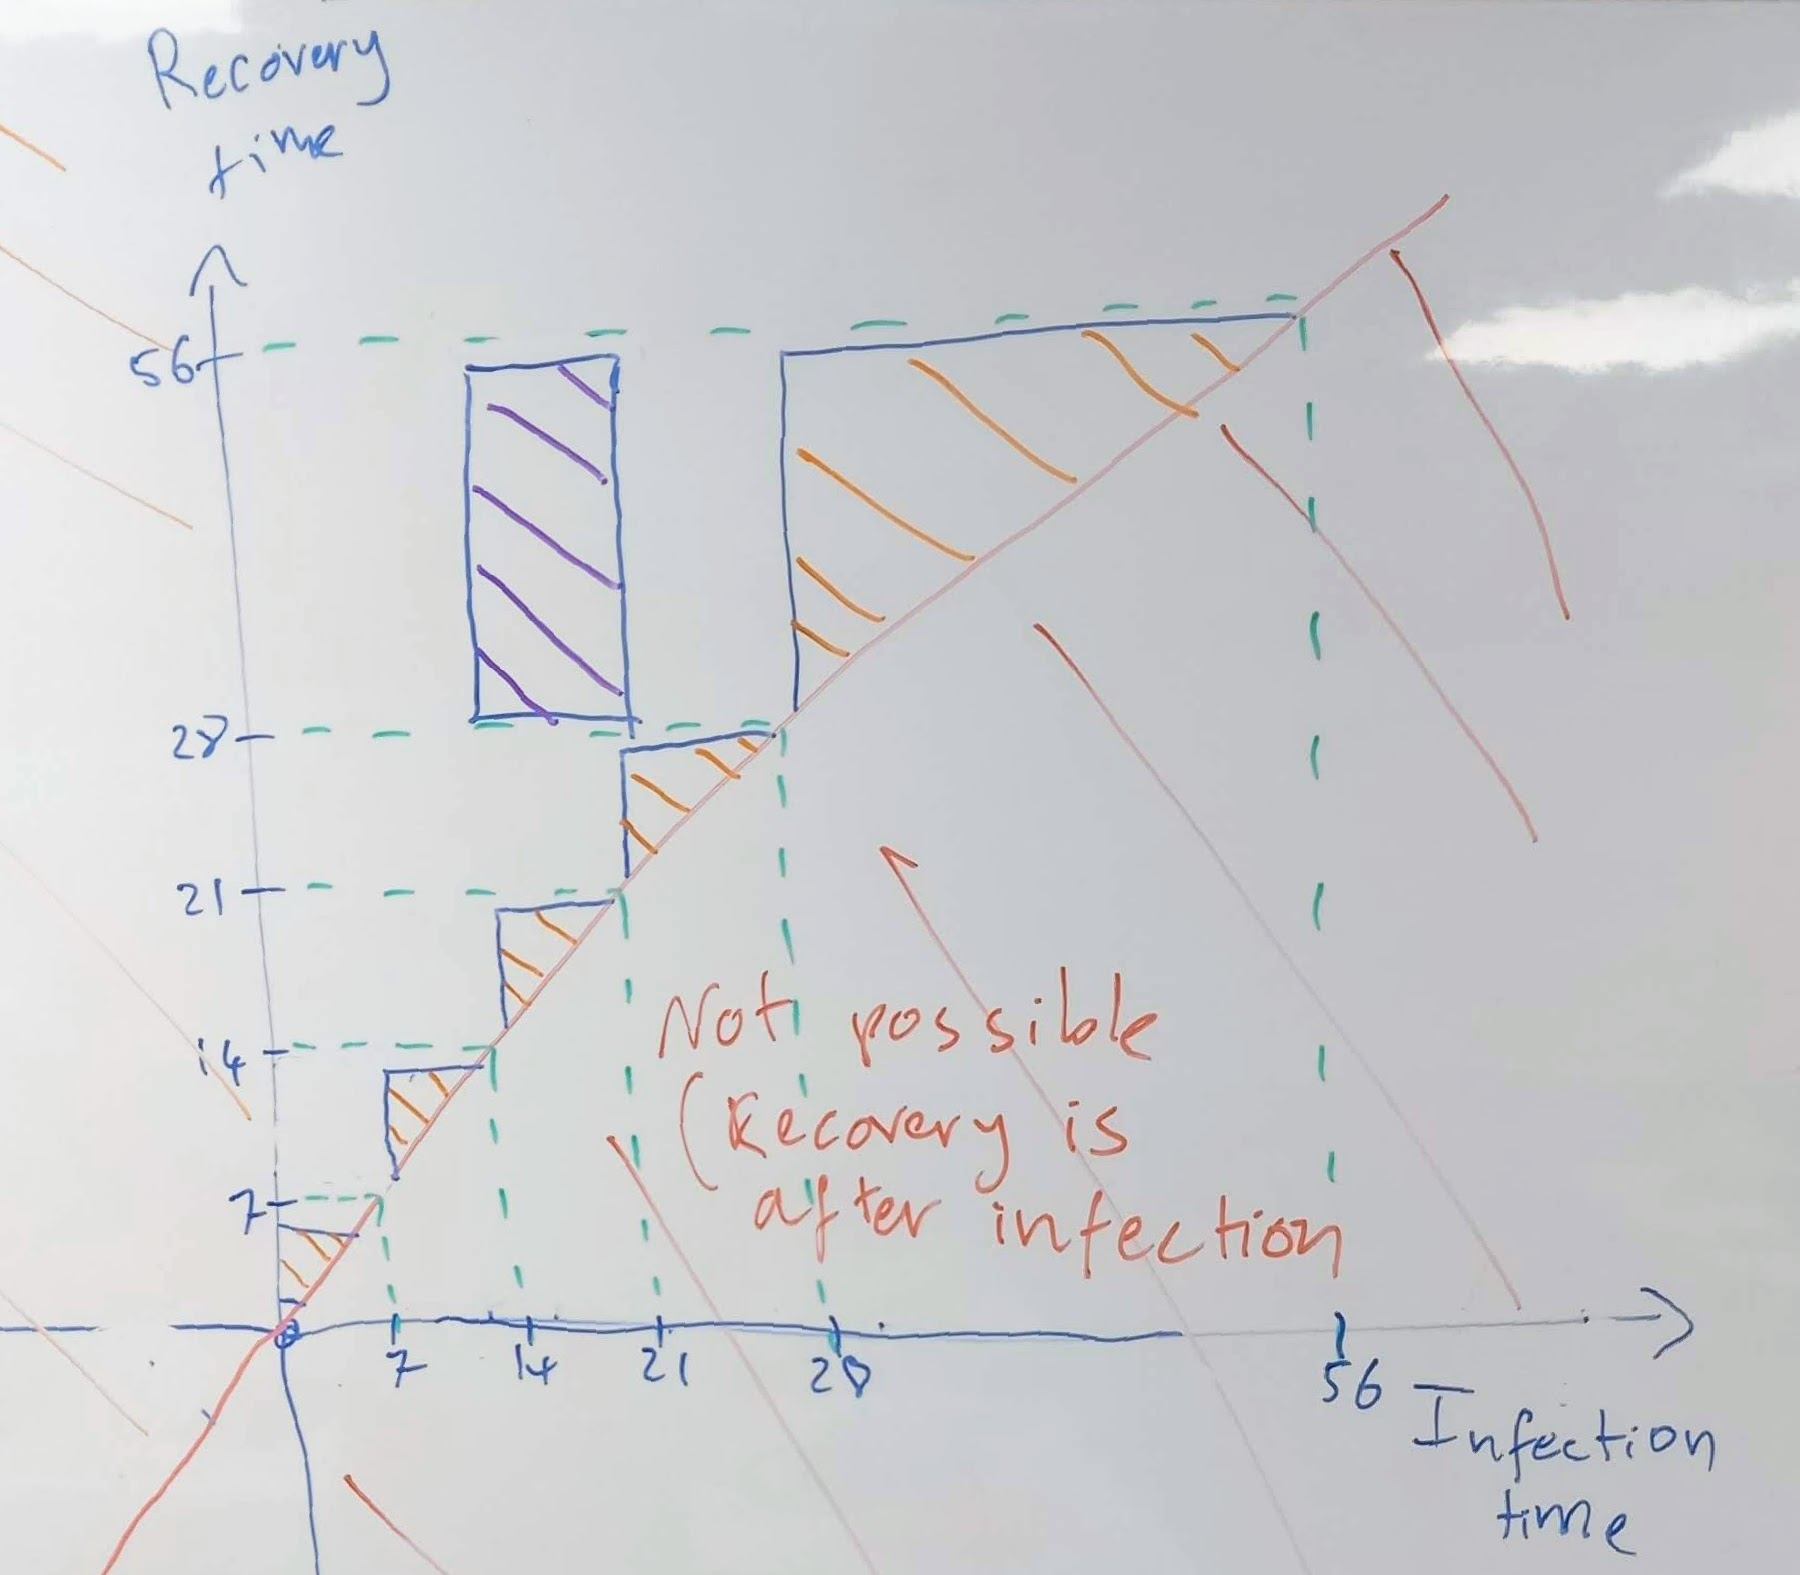
\includegraphics[width=\textwidth]{cis-perfect-testing/images/likelihood_areas.jpg}
\caption{Admissible, $\alpha_i$, inadmissible, $\beta_i$ and
untruncated, $\Omega_i^C$ regions for an episode $i$ in an
individual whose first test was at time 0 and negative, with subsequent
negative tests at times 7, 14, and 56, and positive tests at times 21
and 28. Purple region is $\alpha_i$, orange region (which includes all
negative infection times) is $\Omega_i^C$ and unshaded region is
$\beta_i$.\label{fig:partitionSpace}}
\end{figure}

These three classes span all possible episodes and are mutually
exclusive, and hence the total number of episodes,
$n_i = n_{ia} + n_{iu} + n_{it}$, and
$p_{ia} + p_{iu} + p_{it} = 1$.

Episode $i$ and its ghosts independently occur belong to one of these
classes. Therefore, conditional on $n_i$, the number of episodes in
each class (that is, the counts $n_{ia}, n_{iu}, n_{it}$) are
distributed multinomially. Hence:
\begin{align}
&p(n_{ia} = 1, n_{iu} = 0, n_{it} = n_i - 1 \mid n_i, \theta) \\
&= \frac{n_i!}{n_{ia}! n_{iu}! (n_i- n_{ia} - n_{it})!} p_{ia}^{n_{ia}} p_{ua}^{n_{ia}} p_{it}^{n_i- n_{ia} - n_{it}} \\
&= \frac{n_i!}{(n_i-1)!} p_{ia} p_{it}^{n_i- 1} &\text{as $n_{ia} = 1$ and $n_{iu} = 0$}\\
&= n_i p_{ia} p_{it}^{n_i- 1}
\end{align}

The posterior we are interested in is
$p(\theta \mid n_{ia} = 1, n_{iu} = 0, \dots, n_{n_a,a} = 1, n_{n_a,u} = 0)$,
where $\theta$ are the parameters governing the survival distribution
and hence allow derivation of the $p$s.
\begin{align}
&p(\theta \mid n_{ia} = 1, n_{iu} = 0, \dots, n_{n_a,a} = 1, n_{n_a,u} = 0) \\
&\propto p(\theta) \prod_{i=1}^{n_a} p(n_{ia} = 1, n_{iu} = 0 \mid \theta) \\
&= p(\theta) \prod_{i=1}^{n_a} \sum_{n_i=1}^\infty p(n_{ia} = 1, n_{iu} = 0, n_{it} = n_i - 1 \mid \theta, n_i) p(n_i \mid \theta) \\
&= p(\theta) \prod_{i=1}^{n_a} \sum_{n_i=1}^\infty n_i p_{ia} p_{it}^{n_i- 1} p(n_i) \\
&= p(\theta) \prod_{i=1}^{n_a} p_{ia} \sum_{n_i=1}^\infty n_i p_{it}^{n_i- 1} p(n_i)
\end{align}
where the last line follows by assuming prior independence.

In the following sections, we derive the expressions for $p_{ia}$ and
$p_{it}$ in terms of the data, and analytical solutions for the sum
under different priors.

\subsubsection{Solution for the sum}\label{solution-for-the-sum}

This section is concerned with finding analytical solutions to
$\sum_{n_i=1}^\infty n_i p_{it}^{n_i- 1} p(n_i)$ under two different
assumptions for $p(n_i)$. First, we consider the improper prior
$p(n_i) \propto 1/n_i$ which has several convenient properties. Then,
we consider a negative binomial distribution (including the geometric
and Poisson distributions as a special and limiting case respectively).

The prior $p(n_i) \propto 1/n_i$ means that the model coincides with
the frequentist likelihood-based approach, up to the priors on other
parameters \cites[section 4.2]{dempsterMaximum}{heiseyModelling}[section 8.7.5]{gelmanBayesian}, and is
the reference prior for this quantity\autocite{heBayesiana}. Under this prior,
$\sum_{n_i=1}^\infty n_i p_{it}^{n_i- 1} p(n_i) \propto \sum_{n_i=1}^\infty p_{it}^{n_i-1} = 1/(1-p_{it})$.
% (\protect\hyperlink{ref-dempsterMaximum}{Dempster, Laird, and
% Rubin} (\protect\hyperlink{ref-dempsterMaximum}{1977}) section 4.2;
% \protect\hyperlink{ref-heiseyModelling}{Heisey and Nordheim}
% (\protect\hyperlink{ref-heiseyModelling}{1995});
% \protect\hyperlink{ref-gelmanBayesian}{Gelman et al.}
% (\protect\hyperlink{ref-gelmanBayesian}{2013}) section 8.7.5)

Now consider $N_i \sim \text{NegBin}(\mu, r)$ using the
mean/dispersion parameterisation of the negative binomial. Equivalently:
\begin{align}
N_i \mid \lambda &\sim \text{Poisson}(\lambda) \\
\lambda &\sim \text{Gamma}(a, b)
\end{align}
where $b = r / \mu$ and $a = r$.
Hence:
\begin{align}
\sum_{n_i=1}^\infty n_i p_{it}^{n_i- 1} p(n_i) 
&= \int \sum_{n_i=1}^\infty n_i p_{it}^{n_i- 1} p(n_i \mid \lambda) p(\lambda) d\lambda \\
&= \int \sum_{n_i=1}^\infty n_i p_{it}^{n_i- 1} \frac{\lambda^{n_i} e^{-\lambda}}{n_i!} p(\lambda) d\lambda \\
&= \int e^{-\lambda} \sum_{n_i=1}^\infty p_{it}^{n_i- 1} \frac{\lambda^{n_i-1}\lambda }{(n_i-1)!} p(\lambda) d\lambda \\
&= \int e^{-\lambda} \lambda p(\lambda) \sum_{n_t=0}^\infty p_{it}^{n_t} \frac{\lambda^{n_t} }{n_t!} d\lambda &n_t = n_i - 1 \\
&= \int e^{-\lambda} \lambda p(\lambda) e^{p_{it}\lambda} d\lambda &\text{Poisson pmf} \\
&= \int e^{\lambda (p_{it} - 1)} \lambda p(\lambda) d\lambda \\
&= \int e^{\lambda (p_{it} - 1)} \frac{b^a}{\Gamma(a)} \lambda^{a-1} e^{-b\lambda} \lambda d\lambda \\
&= \frac{\Gamma(a+1)b^a}{\Gamma(a) (b+1-p_{it})^{a+1}} \\ 
  &\; \times \int \frac{(b+1-p_{it})^{a+1}}{\Gamma(a+1)} \\
  &\; \lambda^{(a+1)-1} e^{-(b+1-p_{it})\lambda} d\lambda \\
&= \frac{\Gamma(a+1)b^a}{\Gamma(a) (b+1-p_{it})^{a+1}} &\text{as gamma pdf} \\
&\propto (b+1-p_{it})^{-(a+1)} \\
&= (r/\mu+1-p_{it})^{-(r+1)} \\
&\propto (r+\mu (1-p_{it}))^{-(r+1)}
\end{align}
Note that $r=0$ recovers the previous derivation (up to
proportionality).

The above allows us to sample from the posterior without needing to
sample the $n_i$s. This is convenient because there are as many
$n_i$s as episodes observed and hence is computationally costly to
sample. Furthermore, each $n_i$ is a discrete parameter, and hence
cannot be sampled within the current Stan implementation.

Having estimated the posterior of the other parameters, we might want to
consider the posterior of $n_i$ (normally for diagnostic or model
debugging purposes), which we can sample from the full conditional.
Specifically, for each posterior sample of $\theta$, we sample one
draw from $n_i \mid \theta, y$ where $y$ represents all the data.

Due to the conditional independence of the $n_i$s, we find that:
\begin{align}
&p(n_i \mid \theta, n_{ia} = 1, n_{iu} = 0) \\
&\propto p(n_{ia} = 1, n_{iu} = 0, n_{it} = n_i - 1 \mid n_i, p_{iu}, p_{ia}, p_{it}) p(n_i) \\
&\propto n_i p_{it}^{n_i- 1} p(n_i)
\end{align}
With the prior, $p(n_i) \propto 1/n_i$ then this is a geometric
distribution with parameter $1 - p_{it}$. With a negative binomial
prior, we have:
\begin{align}
n_i p_{it}^{n_i- 1} p(n_i)
&\propto n_i p_{it}^{n_i- 1} \frac{\Gamma(r + n_i)}{n_i!} \left( \frac{\mu}{r+\mu} \right)^{n_i} \\
&\propto \frac{\Gamma((r + 1) + (n_i - 1))}{(n_i-1)!} \left( \frac{\mu p_{it}}{r+\mu} \right)^{n_i-1}
\end{align}
which is a negative binomial pmf with size parameter $r+1$ and
probability parameter $\frac{r + \mu (1 - p_{it})}{r+\mu}$. The mean
of this is
\begin{align}
\frac{(r+1)\mu p_{it}}{r+\mu(1-p_{it})}
\end{align}

\subsubsection{Derivations of probabilities} \label{sec:deriv-probs}

By definition, we have
\begin{align}
p_{ia} &= \prob((b, e) \in \alpha_i) \\
\alpha_i &= \{ (b, e) : l_i^{(b)} \leq b \leq r_i^{(b)} \wedge l_i^{(e)} \leq e \leq r_i^{(e)}\}.
\intertext{Hence:}
p_{ia}
&= \prob \left( l_i^{(b)} \leq B_i \leq r_i^{(b)}, l_i^{(e)} \leq E_i \leq r_i^{(e)} \right) \\
&= \prob \left( l_i^{(e)} \leq E_i \leq r_i^{(e)} \mid l_i^{(b)} \leq B_i \leq r_i^{(b)} \right) \prob \left( l_i^{(b)} \leq B_i \leq r_i^{(b)} \right) \\
&=\sum_{b = l_i^{(l)}}^{r_i^{(b)}} \prob \left( l_i^{(e)} \leq E_i \leq r_i^{(e)} \mid B_i = b \right) \prob \left(B_i = b \right) \\
&=\sum_{b = l_i^{(b)}}^{r_i^{(b)}} \prob \left( l_i^{(e)} - b + 1 \leq D_i \leq r_i^{(e)} - b + 1 \right) \prob \left(B_i = b \right) \\
&=\sum_{b = l_i^{(b)}}^{r_i^{(b)}} \left( S_\theta(l_i^{(e)} - b + 1) - S_\theta(r_i^{(e)} - b + 2) \right) \prob \left(B_i = b \right) \\
&\propto \sum_{b = l_i^{(b)}}^{r_i^{(b)}} \left( S_\theta(l_i^{(e)} - b + 1) - S_\theta(r_i^{(e)} - b + 2) \right)
\end{align}
under the assumption of uniform probability of infection time.

Next, we derive $p_{it} = \prob((b, e) \in \Omega^C_i)$, the probability
that episode $i$ was truncated. A truncated episode means that no test
was performed during the episode or there was no negative test prior to
the episode. Denote by $t_i$ the set of testing times for the
individual in which episode $i$ was observed, and define the time
until the next test on the individual after time $t'$ as:
\begin{align}
t^N_{it} &= \min \{ t' \in t_i : t' \geq t \} - t.
\intertext{Then:}
\Omega^C_i
&= \{ (b, e) : \nexists t \in t_i. b \leq t \leq e \vee b \leq \min(t_i) \} \\
&= \{ (b, e) : e - b < t^N_{ib} \vee b \leq \min(t_i) \}.
\intertext{Hence:}
1 - p_{it}
&= 1 - \prob(E_i - B_i < t_{iB_i}^N \vee B_i \leq \min(t_i)) \\
&= 1 - \prob(E_i - B_i < t_{iB_i}^N \wedge B_i > \min(t_i)) - \prob(B_i \leq \min(t_i)) \\
&= 1 - \sum_{b=\min(t_i) + 1}^T \prob(E_i - b + 1 < t_{ib}^N \mid B_i = b) \prob(B_i = b) \\
  &\; - \sum_{t=1}^{\min(t_i)} \prob(B_i = b)\\
&= 1 - \frac{1}{T} \sum_{b=\min(t_i)+1}^T (1 - S_\theta(t_{ib}^N + 1)) - \frac{\min(t_i)}{T} \\
&= 1 - \frac{T-\min(t_i)}{T} + \frac{1}{T} \sum_{b=\min(t_i)+1}^T S_\theta(t_{ib}^N + 1)) - \frac{\min(t_i)}{T} \\
&= \frac{1}{T} \sum_{b=\min(t_i)+1}^T S_\theta(t_{ib}^N + 1)
\end{align}

\subsection{Full posterior}\label{full-posterior}

Under the prior $p(n_i) \propto 1/n_i$:
\begin{align}
&p(\theta \mid n_{ia} = 1, n_{iu} = 0, \dots, n_{n_a,a} = 1, n_{n_a,u} = 0) \\
&\propto p(\theta) \prod_{i=1}^{n_a} p_{ia} \sum_{n_i=1}^\infty n_i p_{it}^{n_i- 1} p(n_i) \\
&= p(\theta) \prod_{i=1}^{n_a} \frac{p_{ia}}{1-p_{it}} \\
&\propto p(\theta) \prod_{i=1}^{n_a} \frac{\sum_{b = l_i^{(b)}}^{r_i^{(b)}} \left( S_\theta(r_i^{(e)} - b - 1) - S_\theta(l_i^{(e)} - b - 1) \right)}{\sum_{b=\min(t_i)}^T S_\theta(t_{ib}^N + 1)} \\
\end{align}

Under the prior $N_i \sim \text{NegBinom}(\mu, r)$:
\begin{align}
&p(\theta \mid n_{ia} = 1, n_{iu} = 0, \dots, n_{n_a,a} = 1, n_{n_a,u} = 0) \\
&\propto p(\theta) \prod_{i=1}^{n_a} p_{ia} \sum_{n_i=1}^\infty n_i p_{it}^{n_i- 1} p(n_i) \\
&= p(\theta) \prod_{i=1}^{n_a} \frac{p_{ia}}{(r+\mu (1-p_{it}))^{(r+1)}} \\
&= p(\theta) \prod_{i=1}^{n_a} \frac{\sum_{b=l_i^{(b)}}^{r_i^{(b)}} \left( S_\theta(r_i^{(e)} - b - 1) - S_\theta(l_i^{(e)} - b - 1) \right)}{\left( r+\mu/T \left( \sum_{b=\min(t_i)}^T S_\theta(t_{ib}^N + 1) \right) \right)^{(r+1)}} \\
\end{align}

\section{Total model}\label{total-model}

We now consider all $N$ individuals in the CIS cohort who have at
least one test during the period of interest, this includes those
without an observed infection, and assume that each is equally likely to
be infected. As before, $i = 1, \dots, n_a$ indexes episodes but now
$j = 1, \dots, N$ indexes individuals. All episodes have an associated
individual, each individual may have any number (including 0) episodes.
Admissible regions are only defined for episodes, and have not changed
from the previous section. The truncated region is defined for each
individual, in addition we consider the combined truncated region which
is episodes that would be truncated without conditioning on which
individual the episode occurs in:
$\Omega^C = \{ (b, e, j) : (b, e) \in \Omega_j^C \}$.

Denote by $n_\text{tot}$ the total number of episodes across all $N$
individuals, regardless of whether they are admissible or truncated (we
know there are no inadmissible episodes by definition).

For any infection, the probability of it being admissible for episode
$i$ is $\frac{1}{N} p_{ia}$. That is, the probability that the
infection occurs in the individual corresponding to the individual in
which episode $i$ ($1/N$ by the assumption that episodes are equally
likely to occur in any of the $N$ individuals) multiplied by the
probability that the episode is admissible for episode $i$ conditional
on it occurring in the relevant individual ($p_{ia}$).

The total number of truncated infections that occur is
$n_t = n_\text{tot} - n_a$. Conditional on an infection occurring in
individual $j$, its probability of being truncated is $p_{jt}$ (as
defined previously). Therefore, the overall probability of an episode
being truncated is $p_t = \frac{1}{N} \sum_{j=1}^N p_{jt}$.

Consider our data as there being one admissible episode for each
observed episode, and all other episodes being truncated. As in the
previous section, conditional on $n_\text{tot}$, we have a multinomial
likelihood.
\begin{align}
p(\text{data} \mid \theta)
&= \sum_{n_\text{tot}=n_a}^\infty p(\text{data} \mid n_\text{tot}, \theta) p(n_\text{tot}) \\
&= \sum_{n_\text{tot}=n_a}^\infty \frac{n_\text{tot}!}{(n_\text{tot}-n_a)!} \left( \prod_{i=1}^{n_a} \frac{1}{N} p_{ia} \right) p_t^{n_\text{tot}-n_a} p(n_\text{tot}) \\
&= \left( \prod_{i=1}^{n_a} \frac{1}{N} p_{ia} \right) \left( \sum_{n_\text{tot}=n_a}^\infty \frac{n_\text{tot}!}{(n_\text{tot}-n_a)!} p_t^{n_\text{tot}-n_a} p(n_\text{tot}) \right) \\
\end{align}

In this case, it would be computationally feasible to augment the data
with $n_\text{tot}$ directly (as it is only a single parameter).
However, implementation is easier if we can use a closed-form for the
sum (as in the previous section) as it allows the use of standard
implementations of NUTS such as Stan, which cannot handle discrete
parameters.

Assuming $N_\text{tot} \sim \text{NegBin}(\mu, r)$:
\begin{align}
&\sum_{n_\text{tot}=n_a}^\infty \frac{n_\text{tot}!}{(n_\text{tot}-n_a)!} p_t^{n_\text{tot}-n_a} p(n_\text{tot}) \\
&= \int \sum_{n_\text{tot}=n_a}^\infty \frac{n_\text{tot}!}{(n_\text{tot}-n_a)!} p_t^{n_\text{tot}-n_a} p(n_\text{tot} \mid \lambda) p(\lambda) d\lambda \\
&= \int \sum_{n_\text{tot}=n_a}^\infty \frac{n_\text{tot}!}{(n_\text{tot}-n_a)!} p_t^{n_\text{tot}-n_a} \frac{\lambda^n_\text{tot} e^{-\lambda}}{n_\text{tot}!} p(\lambda) d\lambda \\
&= \int \sum_{n_\text{tot}=n_a}^\infty \frac{1}{(n_\text{tot}-n_a)!} p_t^{n_\text{tot}-n_a} \lambda^{n_\text{tot}-n_a} \lambda^{n_a} e^{-\lambda} p(\lambda) d\lambda \\
&= \int \lambda^{n_a} e^{-\lambda} p(\lambda) \sum_{n_t=0}^\infty \frac{1}{n_t!} p_t^{n_t} \lambda^{n_t} d\lambda &n_t = n-n_a\\
&= \int \lambda^{n_a} e^{-\lambda} p(\lambda) e^{\lambda p_t} d\lambda \\
&= \int \lambda^{n_a} e^{-\lambda(1 - p_t)} p(\lambda) d\lambda \\
&= \int \lambda^{n_a} e^{-\lambda(1 - p_t)} \frac{b^a}{\Gamma(a)} \lambda^{a-1} e^{-b\lambda} \lambda d\lambda \\
&= \int \frac{b^a}{\Gamma(a)} \lambda^{a+n_a-1} e^{-(b+1-p_t)\lambda} \lambda d\lambda \\
&= \frac{b^a}{\Gamma(a)} \frac{\Gamma(a+n_a)}{(b+1-p_t)^{a+n_a}} \\
&\propto (b+1-p_t)^{-(a+n_a)} \\
&= (r/\mu + 1 - p_t)^{-(r+n_a)} \\
&\propto(r + \mu (1- p_t))^{-(r+n_a)}
\end{align}

Which gives the full posterior density as:
\begin{align}
p(\theta \mid \text{data})
&\propto \frac{p(\theta) \prod_{i=1}^{n_a} p_{ia}}{(r + \mu(1 - p_t))^{r+n_a}}
\end{align}

As before, being able to reconstruct the posterior of $n_\text{tot}$
using its full conditional is useful.
\begin{align}
p(n_\text{tot} \mid \text{data}, \theta)
&\propto p(\text{data} \mid \theta, n_\text{tot}) p(n_\text{tot}) \\
&= \frac{n_\text{tot}!}{(n_\text{tot}-n_a)!} \left( \prod_{i=1}^{n_a} \frac{1}{N} p_{ia} \right) p_t^{n_\text{tot}-n_a} p(n_\text{tot}) \\
&\propto \frac{n_\text{tot}!}{(n_\text{tot}-n_a)!} p_t^{n_\text{tot}} \frac{\Gamma(r + n_\text{tot})}{n_\text{tot}!} \left( \frac{\mu}{r + \mu} \right)^{n_\text{tot}}  \\
&\propto \frac{\Gamma(r + n_\text{tot})}{(n_\text{tot}-n_a)!} \left( \frac{\mu p_t}{r + \mu} \right)^{n_\text{tot}}  \\
&\propto \frac{\Gamma((r + n_a) + (n_\text{tot}- n_a))}{(n_\text{tot}-n_a)!} \left( \frac{\mu p_t}{r + \mu} \right)^{n_\text{tot}-n_a}  \\
\end{align}
which is a negative binomial pmf with size parameter $r + n_a$ and
probability parameter $\frac{r+\mu(1-p_t)}{r+\mu}$.

\section{False negatives}\label{false-negatives}

In this section, we relax the assumption of perfect testing to allow
some false negatives. We use a fairly simplified model to ensure the
likelihood is tractable. This requires modifying both $p_{ia}$ to
allow for the episode possibly being longer than observed, and
$p_{it}$ to allow for additional episodes being missed.

Specifically, we introduce a constant test sensitivity $p_\text{sens}$
such that:
\begin{align}
\prob(y_i(t) = 1) = \begin{cases} p_\text{sens} &b_i \leq t \leq e_i \\ 0 &\text{otherwise.}\end{cases}
\end{align}

In practice, it is likely that the test sensitivity is a function of the
viral load of an individual (the concentration of viral material in the
part of the body being sampled). For this initial attempt at modelling
the sensitivity, we ignore this complication.

\subsection{Modifying $p_{ia}$} \label{modifying-p_ia}

The idea when modifying $p_{ia}$ is to allow for the negative test
following the last positive to be either a true or false negative. If it
is a true negative, then we have a bound on the length of the episode.
If it is a false negative, then we consider the episode's length
right-censored. The likelihood contribution for an episode is then a
mixture of these two scenarios, with the mixture probability determined
by the test sensitivity.

For tractability, we assume that the tests bounding the start of the
infection ($l_i^{(b)}$ and $r_i^{(b)}$) are true results and hence
$b_i \in [l_i^{(b)}, r_i^{(b)}]$. Furthermore, we consider the tests
only between $r_i^{(b)}$ and $l_i^{(e)}$ inclusive (the positive
tests providing a lower bound on the length of the episode). Denote
these tests by
$t'_i = \{ t \in t_i : r_i^{(b)} \leq t \leq l_i^{(e)} \}$ and their
results by $y_i'$. We know that the test results at times in $t_i'$
are either true positives or false negatives. By definition, the test at
$r_i^{(e)}$ is a false negative if and only if $e_i > r_i^{(e)}$. We
proceed by considering the two cases.

First, if $e_i \leq r_i^{(e)}$. In this case, the test at
$r_i^{(e)}$ is a true negative, as are all other tests not in
$t_i'$, and these occur with probability 1.
\begin{align}
&p(y_i', e_i \leq r_i^{(e)} | b_i, p_\text{sens}, \theta) \\
&= p(y_i', l_i^{(e)} \leq e_i \leq r_i^{(e)} | t_i, b_i, p_\text{sens}, \theta) \\ % &\text{as no false positives}
&= p(y_i' \mid l_i^{(e)} \leq e_i \leq r_i^{(e)}, t_i, b_i, p_\text{sens}, \theta) p(l_i^{(e)} \leq e_i \leq r_i^{(e)} | t_i, b_i, p_\text{sens}, \theta) \\
&= \left( \prod_{t \in t_i'} p_\text{sens}^{y_i(t)} (1 - p_\text{sens})^{(1 - y_i(t))} \right) \left( S_\theta(l_i^{(e)} - b_i - 1) - S_\theta(r_i^{(e)} - b_i - 1) \right)
\end{align}

Second, if $e_i > r_i^{(e)}$. In this case, the test at
$r_i^{(e)}$ is a false negative, occurring with probability
$(1 - p_\text{sens})$, and we have no upper bound on the end of the
infection.
\begin{align}
&p(y_i', e_i > r_i^{(e)} | b_i, p_\text{sens}, \theta) \\
&= p(y_i \mid e_i > r_i^{(e)}, t_i, b_i, p_\text{sens}, \theta) p(e_i > r_i^{(e)} | t_i, b_i, p_\text{sens}, \theta) \\
&= \left( \prod_{t \in t_i'} p_\text{sens}^{y_i(t)} (1 - p_\text{sens})^{(1 - y_i(t))} \right) (1 - p_\text{sens}) S_\theta(r_i^{(e)} - b_i - 1)
\end{align}

Combining the above, the replacement for $p_{ia}$ is:
\begin{align}
p_{ia}'
&= p(y_i' \mid p_\text{sens}, \theta) \\
&= \sum_{b_i = l_i^{(b)}}^{r_i^{(b)}} \left( p(y_i', b_i, e_i \leq r_i^{(e)} \mid p_\text{sens}, \theta) p(y_i', b_i e_i > r_i^{(e)} \mid p_\text{sens}, \theta) \right) p(b_i \mid p_\text{sens}, \theta) \\
&= \left( \prod_{t \in t_i'} p_\text{sens}^{y_i(t)} (1 - p_\text{sens})^{(1 - y_i(t))} \right) \\ & \ \times \sum_{b_i = l_i^{(b)}}^{r_i^{(b)}} \left( S_\theta(l_i^{(e)} - b_i - 1) - S_\theta(r_i^{(e)} - b_i - 1) + (1 - p_\text{sens}) S_\theta(r_i^{(e)} - b_i - 1) \right) p(b_i \mid p_\text{sens}, \theta) \\
&= \left( \prod_{t \in t_i'} p_\text{sens}^{y_i(t)} (1 - p_\text{sens})^{(1 - y_i(t))} \right)\sum_{b_i = l_i^{(b)}}^{r_i^{(b)}} \left( S_\theta(l_i^{(e)} - b_i - 1) - p_\text{sens} S_\theta(r_i^{(e)} - b_i - 1) \right) p(b_i \mid p_\text{sens}, \theta).
\end{align}
Note that if $p_\text{sens} = 1$ then $p_{ia}' = p_{ia}$.

\subsection{Modifying $p_{it}$} \label{modifying-p_it}

With false negatives, an episode with can be truncated in the following
ways:

\begin{enumerate}
\item
  The episode begins before $\min(t_i)$ (assuming there is a
  negligible probability of a false negative test at this point).
\item
  The duration of the episode is less than $t_{ib_i}^N$. These first
  two mechanisms are how truncation previously occurred, with
  probability $p_{it}$.
\item
  The duration of the episode is at least as long as $t_{it}^N$ but
  less than the time to the second test after $t$, $t_{it}^{2N}$,
  and a false negative episode occurred at the first test after $t$.
  This occurs with probability:
  \begin{math}
    (1 - p_\text{sens})\frac{1}{T} \sum_{b=\min(t_i)}^T \left( S_\theta(t_{ib}^N + 1) - S_\theta(t_{ib}^{2N} + 1)\right).
  \end{math}
\item
  The duration of the episode is at least as long as $t_{it}^{2N}$,
  and all the tests within the episode (at least two) are false
  negatives. We assume this occurs with negligible probability.
\end{enumerate}

Hence, the replacement for $1 - p_{it}$ is:
\begin{align}
1 - p_{it}'
&= 1 - p_{it} - (1 - p_\text{sens})\frac{1}{T} \sum_{b=\min(t_i)}^T \left( S_\theta(t_{ib}^N + 1) - S_\theta(t_{ib}^{2N} + 1)\right) \\
&= \frac{1}{T} \sum_{b=\min(t_i)}^T \left( p_\text{sens} S_\theta(t_{ib}^N + 1) + (1 - p_\text{sens}) S_\theta(t_{ib}^{2N} + 1)\right) \\
\end{align}

\end{document}